\newpage
\section{System Specifications}
% This section of the elaborate will involve the discussion of the system requirements, as well as how the system have been designed.
\subsection{System Requirements}
By defining the system functional requirements, the application key functionalities to implement were identified, by considering also existing applications (see \cref{popularApps}) that represent standards on the health and fitness market. Security, usability as well as other important aspects were considered, leading to the definition of the non-functional requirements. The requirements can be classified as follows:
\vspace{5ex}
\begin{table}[h!]
    \setstretch{\myspacing}
    \centering
    \begin{tabular}{|>{\raggedright\arraybackslash}p{0.1\linewidth}|>{\raggedright\arraybackslash}p{0.2\linewidth}|>{\raggedright\arraybackslash}p{0.6\linewidth}|}
        \hline
        \textbf{FR1} & \multicolumn{2}{>{\centering\arraybackslash}p{0.7\linewidth}|}{\textbf{User Management}} \\
        \hline
        FR 1.1 & Registration & Allow a user to register through google or by defining his credentials. Additionally, allow an user to enter his demographics (age,sex,...) and body (height,weight,...) data when the registration is in progress. \\
        \hline
        FR 1.2 & Login Management & Allow a user to log in into his account with the methods that he had setup and allow also to change the password, including the possibility to recover it in case he forgot it.  \\
        \hline
        FR 1.3 & Account Management & Allow a user to log out from his account, delete it as well as add either google or classic credential method as login method, in case he hadn't used before.  \\
        \hline
    \end{tabular}
\end{table}


\begin{table}[h!]
    \setstretch{\myspacing}
    \centering
    \begin{tabular}{|>{\raggedright\arraybackslash}p{0.1\linewidth}|>{\raggedright\arraybackslash}p{0.2\linewidth}|>{\raggedright\arraybackslash}p{0.6\linewidth}|}
        \hline
        \textbf{FR1} & \multicolumn{2}{>{\centering\arraybackslash}p{0.7\linewidth}|}{\textbf{User Management}} \\
        \hline
        FR 1.4 & Home Page & Allow a user to visualize data regarding his steps, food, sleep and emotional state. Also allow to visualize data that exceeds the user goals differently (they visually differ from the other ones). \\
        \hline
        FR 1.5 & Learn Page & Allow the user to take lessons and then related quizzes to assess their preparation on the topic through the learn page. The user can browse the lesson and his topics, then take the corresponding test if he wants. \\
        \hline
        FR 1.6 & Health Measures Page & Allow a user to view his vital metrics by using charts organized in different tabs instead of raw values, for a better understanding. \\
        \hline
        FR 1.7 & Personal Information Page & Allow a user to edit some of his personal measures (provided at registration time) and add his activity goals, used as upper bound into the charts of the Home Page. \\
        \hline
    \end{tabular}
    \caption{Overview of Functional Requirements related to the User Management.}
\end{table}


\begin{table}[h!]
    \setstretch{\myspacing}
    \centering
    \begin{tabular}{|>{\raggedright\arraybackslash}p{0.1\linewidth}|>{\raggedright\arraybackslash}p{0.2\linewidth}|>{\raggedright\arraybackslash}p{0.6\linewidth}|}
        \hline
        \textbf{FR2} & \multicolumn{2}{>{\centering\arraybackslash}p{0.7\linewidth}|}{\textbf{Notification System}} \\
        \hline
        FR 2.1 & Notification System & Allow a user to receive notification with different frequencies to prompt him into inserting data regarding food, emotional aspect, balance capability, strenght capability. \\
        \hline
        FR 2.1 & Notification Parameters & Allow a user to receive notification based on common users parameter, but also personalized based on some personal parameter. \\
        \hline
        FR 2.2 & Body Balance Notification & Allow a user to receive notification to prompt him to insert data regarding his balance capability, such as balance test on one leg at a time or tandem walk. \\
        \hline
        FR 2.3 & Body Strength Notification & Allow a user to receive notification to prompt him to insert data regarding his strenght capability, such as number of squats, abdominals and push ups, as well as a grip strength test. \\
        \hline
        FR 2.4 & Emotional Notification & Allow a user to receive notification to prompt him to insert data regarding his emotional aspect by following the panas guidelines. \\
        \hline
        FR 2.5 & Food Notification & Allow a user to receive notification to prompt him into inserting data regarding his consumed food, with this type of notification being more frequent than the others. \\
        \hline
        FR 2.6 & Assessment & Allow a user to visualize a periodic assessment produced thanks to the data that were previously inserted. \\
        \hline
    \end{tabular}
    \caption{Overview of Functional Requirements related to the Notification System provided to the User.}
    \label{tab:fr2}
\end{table}

\begin{table}[h!]
    \setstretch{\myspacing}
    \centering
    \begin{tabular}{|>{\raggedright\arraybackslash}p{0.1\linewidth}|>{\raggedright\arraybackslash}p{0.2\linewidth}|>{\raggedright\arraybackslash}p{0.6\linewidth}|}
        \hline
        \textbf{FR3} & \multicolumn{2}{>{\centering\arraybackslash}p{0.7\linewidth}|}{\textbf{Data Management}} \\
        \hline
        FR 3.1 & Data Sources & Employing as main app data source Health Connect (Health data management and integration platform developed by Google), while still keeping Google Firebase as additional data source where needed. \\
        % Health Connect and Apple Health (Health data management and integration platforms, developed by Google and Apple respectively),
        \hline
        FR 3.2 & Health Data Source & The system must retrieve and display users' health data relating to steps and sleep on the home page, as well as their heart and lung data in health measures page. \\
        \hline
        FR 3.3 & Google Firebase Data Source & The system must retrieve and display users' health data related to emotional state and food on the home page. Also weight, waist circumference, grip, balance and strenght data are retrieved from this data sources and showed in the health measures page. Finally, profile and goals data are also fetched and showed into personal information page. \\
        \hline
        FR 3.4 & Health Data Backup & The system must add the necessary logic to perform a backup of the users's health data. \\
        \hline
    \end{tabular}
    \caption{Overview of Functional Requirements related to the Data Management.}
    \label{tab:fr3}
\end{table}

\begin{table}[h!]
    \setstretch{\myspacing}
    \centering
    \begin{tabular}{|>{\raggedright\arraybackslash}p{0.1\linewidth}|>{\raggedright\arraybackslash}p{0.2\linewidth}|>{\raggedright\arraybackslash}p{0.6\linewidth}|}
        \hline
        \textbf{FR4} & \multicolumn{2}{>{\centering\arraybackslash}p{0.7\linewidth}|}{\textbf{Admin Management}} \\
        \hline
        FR 4.1 & Admin Application & Allow the admin to use a web application in order to modify system metrics. \\
        \hline
        FR 4.2 & Login/Logout & Allow the admin to login into the web application, as well as to logout. \\
        \hline
        FR 4.3 & Notifications Parameters Edit & Allow the admin to change some of the metrics related to the notification system set up for users. \\
        \hline
        % SE FACCIAMO METTERE
        % FR 4.4 & Application Lessons & Allow the admin to manage the lessons that are provided to the users inside the application. \\
        % \hline
        % FR 4.5 & Application Quizzes & Allow the admin to manage the quizzes that corresponds to the lessons and are provided to the users inside the application. \\
        % \hline
    \end{tabular}
    \caption{Overview of Functional Requirements related to the Web Application provided to the Admin.}
\end{table}

\clearpage

\noindent As far as concerns the non-functional requirements, we can classify them as follows:

\begin{table}[h!]
    \setstretch{\myspacing}
    \centering
    \begin{tabular}{|>{\raggedright\arraybackslash}p{0.1\linewidth}|>{\raggedright\arraybackslash}p{0.2\linewidth}|>{\raggedright\arraybackslash}p{0.6\linewidth}|}
        \hline
        \textbf{NFR} & \textbf{Type} & \textbf{Description} \\
        \hline
        NFR1 & Reliability & The system should ensure at least 80\% accuracy and functionality over the course of a year. \\
        \hline
        NFR2 & Portability & The application must be capable of running on Android devices. \\
        \hline
        NFR3 & Security & Robust login mechanisms should be implemented to protect user data and limit access only to authorized individuals. \\
        \hline
        NFR4 & Usability & The application should be intuitive enough for users of all ages and skill levels, requiring minimal training. \\
        \hline
        NFR5 & Data Privacy & User data must adhere to OAUTH for secure data handling. \\
        \hline
        NFR6 & Performance & The app should smoothly load and handle user interactions within two seconds under typical conditions in order to achieve an optimal user experience. \\
        \hline
        NFR7 & Interoperability & The application should seamlessly connect with third-party platforms like Health Connect and Apple Health, maintaining data accuracy and improving functionality. \\
        \hline
        NFR8 & Localization & The app should support at least English and Italian languages, adapting content and formats (e.g., date, currency) accordingly. \\
        \hline
        NFR9 & Modularity & The app's architecture should support modular development to facilitate future updates without impacting the entire codebase. \\
        \hline
    \end{tabular}
    \caption{Overview of Non-Functional Requirements related to the system.}
    \label{tab:nfr}
\end{table}
\newpage
\subsection{System Design and Architecture}
\subsubsection{System Design}

While designing the system, the main components have been chosen in order to provide a clear and intuitive application system, as well as a robust and secure backend.
\newline For the frontend application part, cross-platform frameworks have been analyzed, having in mind the possibility to extend the application also to IOS platform. Flutter, React Native and Xamarin were considered, but Flutter has been chosen, thanks to the possibility to develop a single codebase for both Android and IOS, and also for his strong support by Google who created it, that makes it a stable and reliable system, as well as a big community and an official package repository where tons of libraries can be found. Considering the web application, among several frameworks available (like React, Angular, Vue.js) React has been chosen, given his diffusion, simplicity and modularity.   
\newline Regarding the backend part, different alternatives were considered, also based on the frontend and our requirements:
\begin{itemize}[nosep] % 'nosep' removes extra spacing between items
    \item \textbf{AWS Amplify}, set of tools and services provided by Amazon Web Services (AWS) to build secure and scalable mobile applications. It comes with a suite of services that streamline the development process, like authentication, storage, GraphQL and REST APIs as well as analytics. 
    \item \textbf{Express}, fast and minimalist web framework built on top of Node.js which is a javascript runtime.
    \item \textbf{Microsoft Azure}, cloud computing service that provides a wide range of cloud services, like analytics, storage, and networking. It allows developers to build, deploy, and manage applications through Microsoft-managed data centers.
    \item \textbf{Spring Boot}, a Java-based framework used to create stand-alone, production-grade applications, which simplifies the development of new applications by providing code and configuration through annotations.
    \item \textbf{Firebase}, comprehensive app development platform by Google that provides a variety of tools and services to help developers build high-quality apps quickly.
\end{itemize}
\newpage
\noindent Among them, Express was immediately discarded despite its simplicity, because it mainly focuses an APIs, does not provide authentication and it is not as rich of services as the others, so it does not fit our needs. Spring Boot was also discarded, given the need to setup external service for authentication (like keycloak IAM) and maintain a server where the backend could run. AWS Amplify and Microsoft Azure were also closer to our needs, but Firebase was chosen, thanks to his Flutter support and seamless integration (since bith made by Google) and thanks to the variety of services it provides: Cloud Firestore as a data source, the Authentication system, Cloud Storage system as well as a suite of analytics service to monitor the application (Analytics, Performance, Crashlytics).
% TODO: se ne parlo mettere Release Monitoring).
\subsubsection{System Architecture}

Focusing on the system architecture, it can consequently be summarized as follows:
\begin{figure*}
    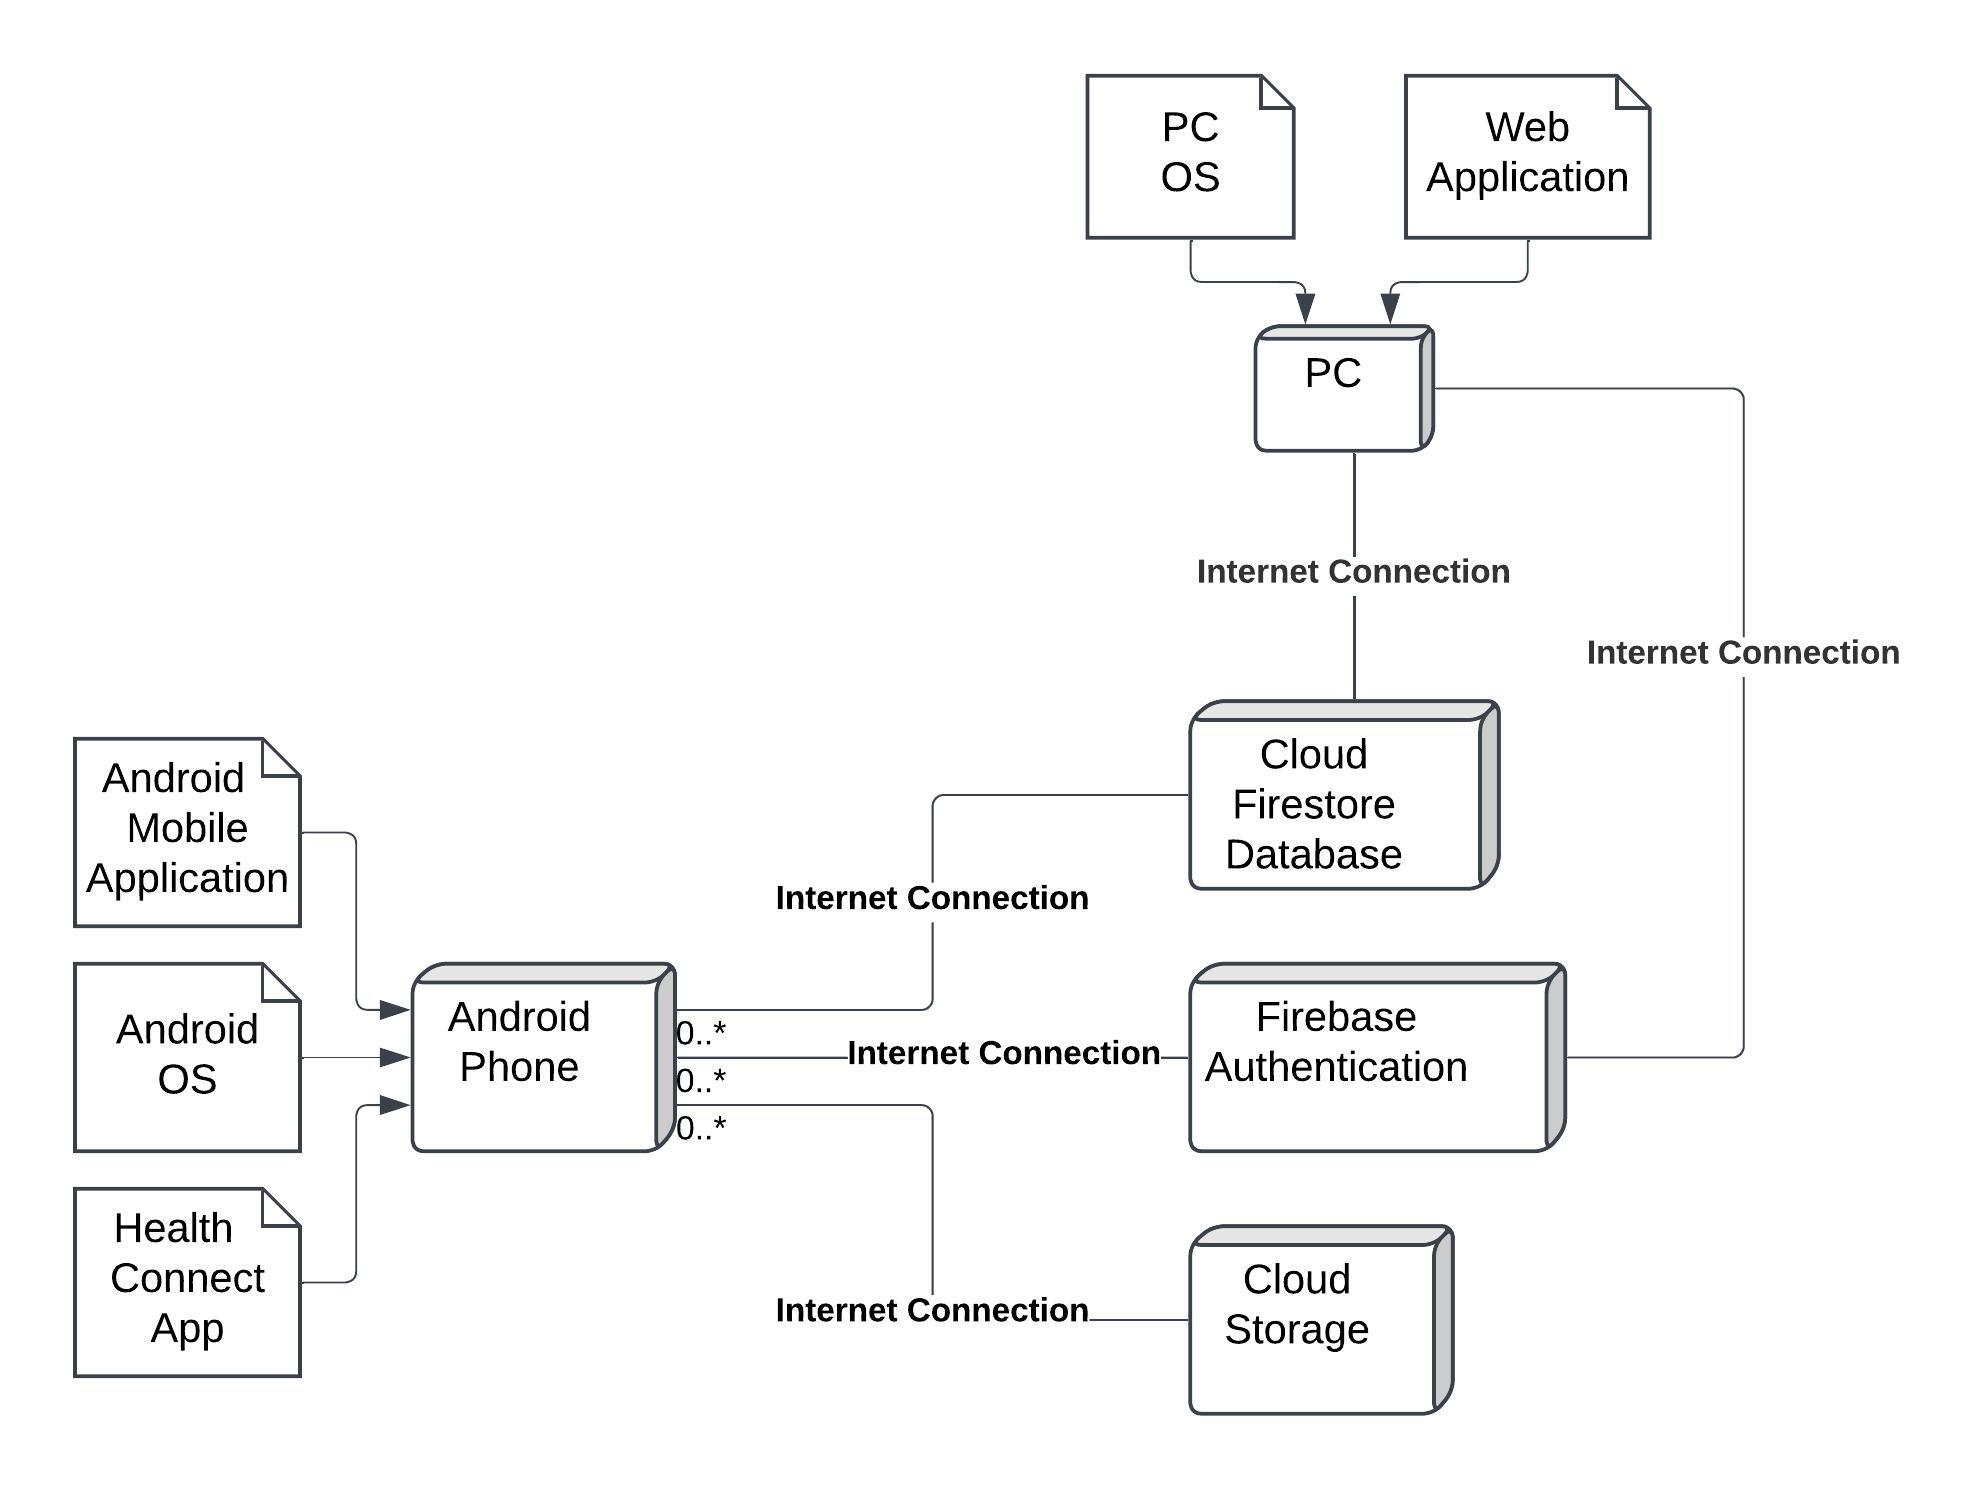
\includegraphics[width=1.0\linewidth]{./images/system_architecture.jpeg}
    \caption{Overview of the System Architecture.}
    \label{fig:systemArchitecture}
\end{figure*}

% \noindent We can clearly distinguish the two main use cases (Android and IOS) with their distinguishing components and the common ones:
\newpage
\noindent We can identify the architecture with the following components:
\vspace{3ex}
\begin{itemize}[nosep] % 'nosep' removes extra spacing between items
    \item \textbf{Android Phone} that represent the physical smartphone, along with his operating system, our application installed and health connect installed, used to manage in an unified way the health data on Android.
    % , that further interacts with google fit server whenever is needed.
    % \item \textbf{Google Fit} server, used among the health connect app data sources.
    \item \textbf{Cloud Firestore Database} server, firebase service employed as a data source for the application logic, containing needed data, such as profile information.
    \item \textbf{Firebase Authentication} server, firebase service employed in order to perform and enforce authentication.
    \item \textbf{Cloud Storage} server, firebase service employed to store the backup of the health data for each user (see \cref{tab:fr3} FR 3.4).
    \item A \textbf{Personal Computer} along with his operating system and a web application that allows to authenticate and to interact with the Cloud Firestore Database on administrator side, in order to modify the system metrics for users notifications, as well as manage lessons and quizzes that are then showed to the users.  
\end{itemize}

\newpage
\noindent In addition to this architecture, the system can be further enriched by integrating a wearable device, that can be a very useful tool to gather data, as previously explained in \cref{sec:wearableDevices}. In this scenario the wearable device will be connected to the smartphone:

\begin{figure*}
    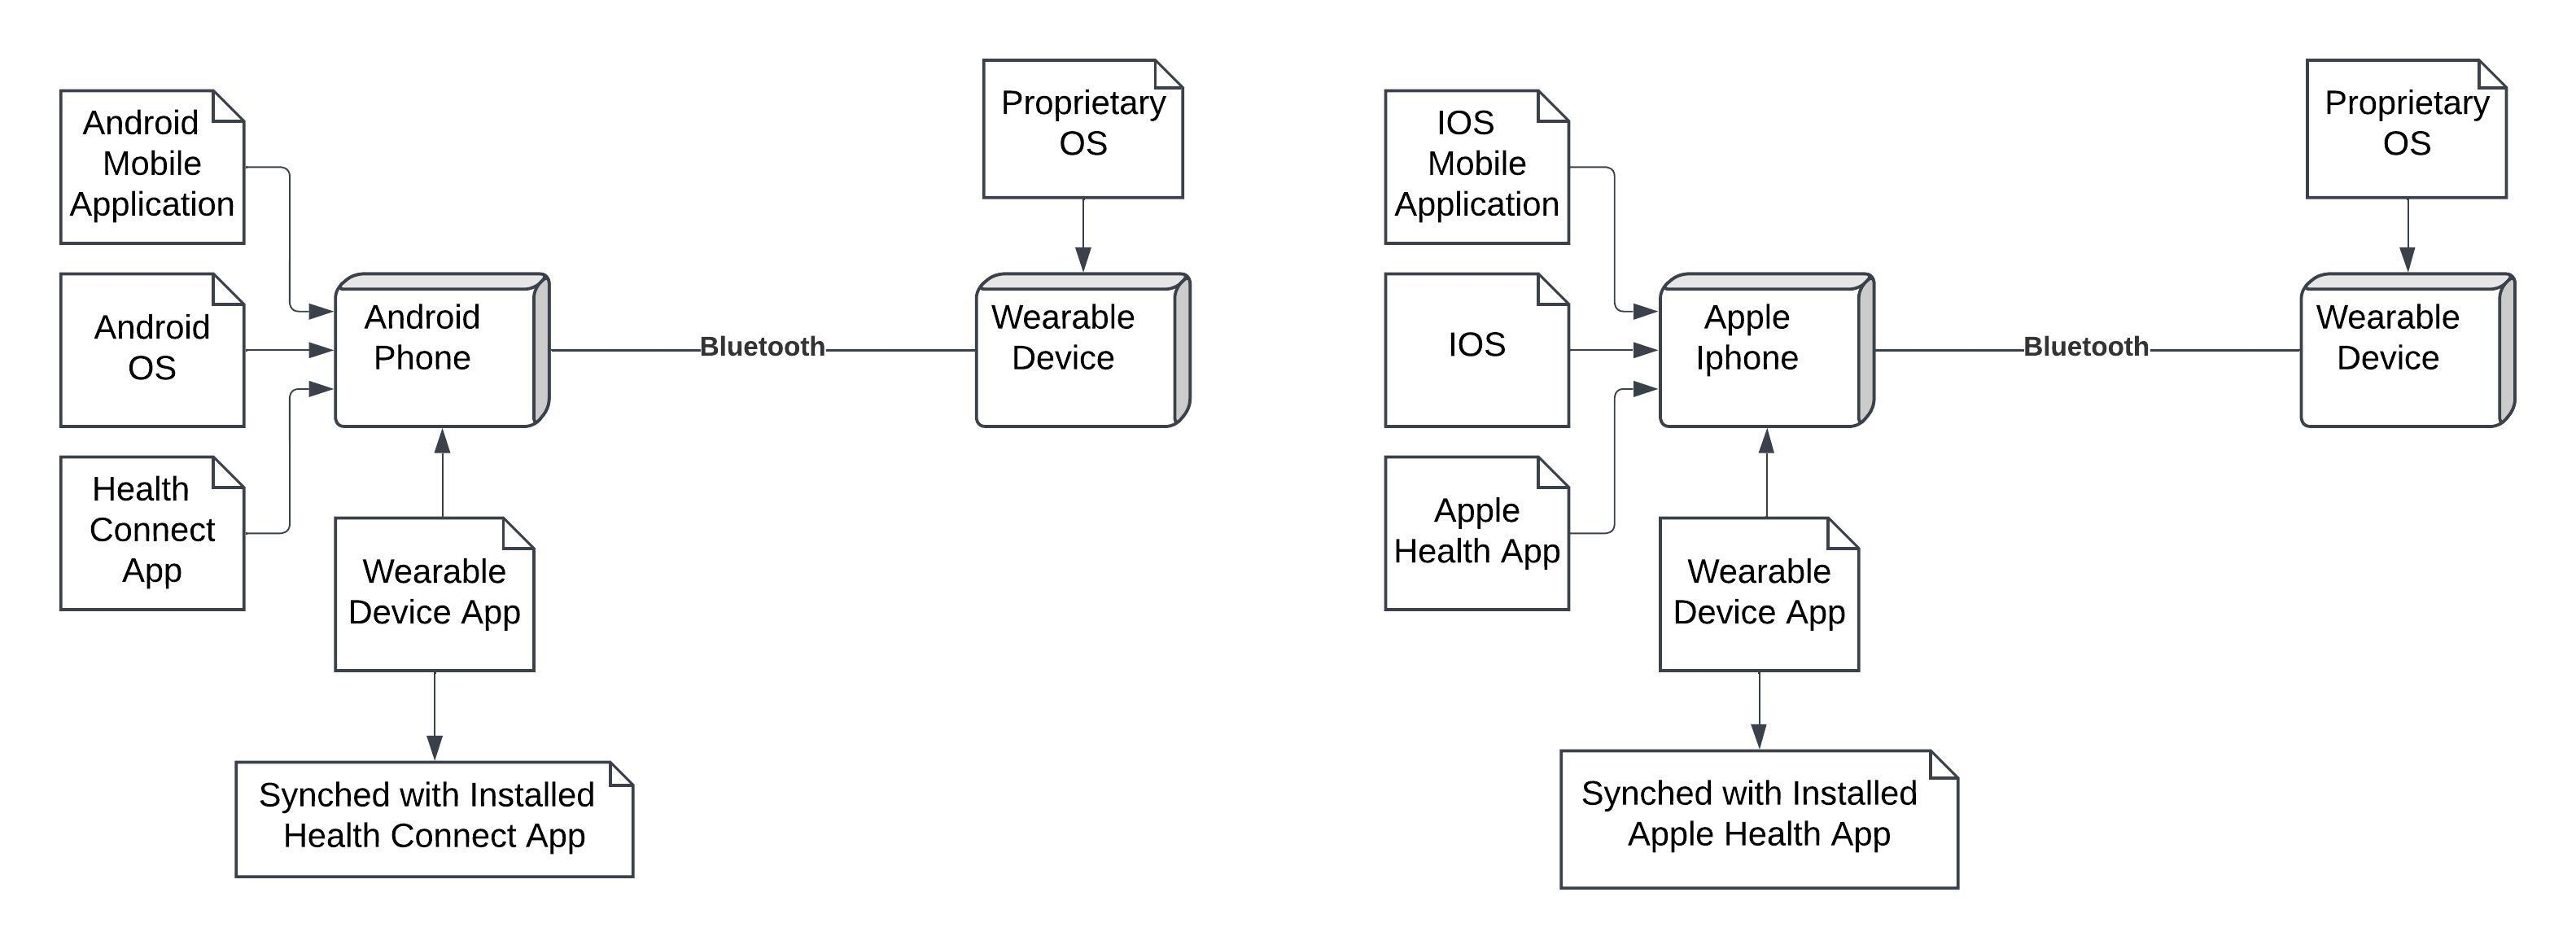
\includegraphics[width=1.0\linewidth]{./images/system_architecture_wearable.jpeg}
    \caption{Overview of the Mobile System Architecture with Wearables.}
    \label{fig:systemArchitectureWearables}
\end{figure*}

\noindent In this case the architecture has been extended with the wearable devices, along with his operating system, that through bluetooth connection can communicate with the smartphone. On the smartphone side, the wearable application will be able to retrieve the data from the wearable device to then sync with the Health Connect data management service.
% \noindent In this case the architecture has been extended with the wearable devices, along with his operating system, that through bluetooth connection can communicate with the smartphone (Android or IOS). On the smartphone side, the wearable application will be able to retrieve the data from the wearable device to then sync with the respective data management service (respectively Health Connect or Apple Health).
\newpage